\myparagraph{Préparation et pré-traitement}
\par L'évaluation de la segmentation avec des vidéos va s'effectuer non pas avec la caméra mais avec un matériel vidéo virtuel. En effet, il n'est pas réaliste de pouvoir travailler sur le terrain. La commande "segnet-camera" permet de fournir en option le matériel qui doit être utilisé, par exmeple "/dev/video0" pour la caméra. Le module "v4l2loopback"\footnote{\url{https://github.com/umlaeute/v4l2loopback}} permet de créer un matériel vidéo virtuel "/dev/video1". Ce matériel permet de recevoir un flux vidéo, qui pourra alors alimenter l'utilitaire "segnet-camera", comme le ferait la caméra. Le flux vidéo sera produit par l'utilitaire "gstreamer" avec comme données d'entrées le fichier de la vidéo et dirigé vers le matériel vidéo virtuel "/dev/video1".
\par La difficulté réside dans le fait que le matériel vidéo virtuel et le flux vidéo doivent être compatible avec ce que l'utilitaire "segnet-camera" s'attend, et qui a été conçut pour être compatible avec une caméra. 
\begin{figure}[H]
    \centering
    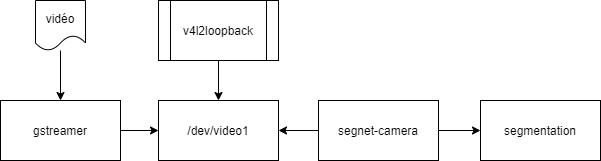
\includegraphics[width=.5\textwidth]{arch_segmentation_video}
    \caption[Diagramme d'architecture de la segmentation d'une vidéo]{Diagramme d'architecture de la segmentation d'une vidéo}
    \label{fig:arch_segmentation_video}
\end{figure}
\myparagraph{Segmentation et évaluation}
{\color{red}décrire la méthodologie utiliser pour exécuter la segmenation de vidéos, quelles vidéos, les résolutions et FPS, les scripts, et l'évaluation\todo{TODO}}